\section{Numeric reference benchmark and transfer limits}
The supplied benchmark contains numeric spectra for nominal Cu(0), Cu(I) in Cu\textsubscript{2}O, and Cu(II) in CuO. Formal oxidation states are chemical labels, not inferred continuous atomic charges. The complete $3\times6$ provenance matrix includes five computational methods and experiment. All three experimental columns are present; Cu\textsubscript{2}O PBE, Cu\textsubscript{2}O ``GW'', and CuO PBE lack usable numeric XAS spectra. Their comparison cells remain blank. Cu\textsubscript{2}O PBE has no dielectric XAS block; the CuO PBE XAS output is incomplete; no Cu\textsubscript{2}O ``GW'' XAS OUTCAR was supplied. A zero-byte Cu\_PBE.dat is preserved as supplied, but the metallic PBE series is recovered from its actual OUTCAR.

The original Cu\_XAS.ipynb is preserved byte for byte. All seven cells are audited. Cells 1--2 specify Gaussian $\sigma=1$~eV; cells 1--5 use inconsistent $+120$, $+124$, $+125$, $-8$, and $-9$~eV offsets. Later cells reuse the variable intensity\_broad across different calculations, and the empty PBE export prevents a clean execution of the original notebook. These plotting choices are not adopted as measured instrumental widths or validated energy calibrations. The orphan Cu\_GW.dat export is retained but cannot be traced to the supplied OUTCAR arrays; it is not substituted for a verified calculation. The revised notebook executes the portable processing script and displays provenance, settings, metrics and all four reference grids.

\subsection{Backend identity and native processing}
The Cu metal folder labels agree with its FDMNES input modes, but the Cu\textsubscript{2}O and CuO folder names are reversed. Classification uses the Green keyword and the finite-difference output banner, retaining the original paths in provenance. The reference FDMNES logs identify revision 11 April 2025, radius 7~\AA, SCF and Perdew. Five completed native convolutions report Gamma\_hole $=1.55$~eV, Gamma\_max $=15$~eV, Ecent $=30$~eV and Elarg $=30$~eV. These are separate from the ML archive's Gamma\_max $=10$~eV records. The native energy-dependent convolution is retained without a second lifetime convolution or an assumed redefinition of its widths. CuO Green includes two symmetry-inequivalent site contributions in its native convolution. Its native site shifts are retained.

The CuO finite-difference output in the folder named fdm\_green is a single saved site-1 raw absorption curve and has no completed convolution in the available log. It receives only the explicit constant core-lifetime prescription below; missing final-state broadening is a limitation, not an inferred default. FEFF 9.6.4 outputs already include intrinsic lifetime and self-energy treatment (Gam\_ch $=1.729$~eV in their headers); no additional lifetime is applied. FEFF uses column omega and absorption mu, not its relative-energy column. The preserved inputs use COREHOLE RPA, SCF radius 7~\AA, and FMS radius 9~\AA.

The VASP 6.3.2 XAS arrays are the diagonal trace divided by three of the imaginary dielectric function. Off-diagonal tensor components are excluded; this is an isotropic tensor average for the designated core-hole atom, not a multisite absorber average. Inputs specify ICORELEVEL $=2$, CH\_LSPEC and CH\_SIGMA $=0.1$~eV. Their folder names do not demonstrate GW or electron--hole ladder calculations. The CH\_SIGMA documentation describes built-in Gaussian broadening; its exact sigma/FWHM convention is not independently established for this executable. We preserve it without another primary Gaussian or deconvolution. Ground-state smearing SIGMA is not a measured spectral resolution.

\subsection{Explicit additional broadening and normalization}
For VASP and unconvolved CuO FDM only, an explicit constant Lorentzian core-lifetime comparison prescription uses FWHM $1.55$~eV, equivalently HWHM $\gamma=0.775$~eV, with kernel $\gamma/[\pi(\Delta E^2+\gamma^2)]$. The chosen number uses the Cu K lifetime parameter in the supplied FDMNES logs as a comparison estimate; it is not a claim that a matching source establishes that parameter's version-specific width convention. Quadrature uses the native energy spacing and renormalizes finite-domain kernel weights. Raw and broadened arrays are saved separately. This constant treatment cannot reconstruct the missing CuO final-state loss function. The two endpoint samples at the same energy in a native output are averaged, with the original preserved.

No measured instrumental resolution is available, so the primary added Gaussian has $\sigma=0$~eV (FWHM 0). A separate sensitivity plot adds the original notebook's unvalidated $\sigma=1$~eV, FWHM $2\sqrt{2\ln2}\sigma=2.35482$~eV. It is not fitted, is not called a measured resolution, and does not replace the primary curves. Existing native convolutions remain intact. No width is optimized against experiment.

The processing order is parsing, tensor/duplicate averaging, the explicitly remaining lifetime treatment, fixed background/scale determination, energy shift, and interpolation on supported common windows. A constant local pre-edge mean is subtracted and the local post-minus-pre jump divides the curve. The reference pre/post windows are 8974--8976 and 9020--9028~eV. Full conventional long-range pre-edge regression is unsupported for the FDMNES arrays, which begin at 8974~eV. Consequently these are conditional local edge-jump comparisons, not standardized absolute accuracy measurements. No missing long-range background is extrapolated.

For calculations without an absolute calibration, fixed source windows are selected once, before fitting any shift. FDMNES uses the above windows directly. FEFF uses 8986--8988 and 9032--9040~eV (nominal $-12$~eV normalization axis); the former is below its native Fermi-level threshold. VASP PBE uses 8854--8856 and 8900--8908~eV (nominal $+120$~eV); the ``GW'' alias uses 8844--8846 and 8890--8898~eV (nominal $+130$~eV), below its first numeric onset for the pre-edge window. These nominal offsets select normalization intervals only and are distinct from fitted calibration. The source-point counts, backgrounds and jumps are recorded in normalization.csv; inadequate windows are recorded rather than extrapolated. The experimental export appears already merged/normalized, but its upstream processing and polarization are not reported. Its metallic column identifies a 100~nm Cu electrode at $-0.4$~V, not a certified bulk foil. These limitations constrain transfer conclusions.

This reference normalization is distinct from the archived ML minimum-subtracted unit-area representation; no ML preprocessing, measurement array, prediction or score was altered.

\subsection{Energy alignment, metrics and computational cost}
The sign convention is $E_{\rm plotted}=E_{\rm input}+\Delta E$. Experiment retains its supplied photon-energy column. A single calibration shift is fitted on metallic Cu for each backend, shared across compounds, with both FDMNES modes sharing the Green-derived shift. Bounds are $[-20,20]$~eV (FDMNES), $[-25,25]$~eV (FEFF), and $[0,200]$~eV (VASP). The objective is normalized RMSE on 8980--9020~eV with 0.2~eV linear sampling. A 0.25~eV coarse scan precedes bounded scalar refinement. There is one fitted calibration parameter per backend; normalization and widths are fixed. Separately aligned shape views permit one residual compound/method shift within $\pm20$~eV of the common offset. They remove chemical-shift information and must not be used as evidence of absolute energy agreement. No per-peak warping is performed.

Metrics use only intersection support and never extrapolate. RMSE is in experimental local-edge-jump units, correlation is omitted when variance is inadequate, and global-peak differences are omitted for ambiguous/endpoint maxima. A unique edge assignment is not robust for these short, multi-maximum curves, so edge-position differences remain unreported. Every comparison records its actual window and point count; the common-offset comparisons have 201 samples. Native-axis VASP metrics can have insufficient or only tail overlap and cannot establish absolute agreement.

\small\begin{longtable}{lllrrrr}
\caption{Complete available reference-v2 similarities. C: Cu-calibrated; S: compound shape alignment; G: added Gaussian diagnostic; N: native axis. All windows are 8980--9020 eV, 201 points. Full units, widths, settings and shifts are also in similarity\_metrics.csv.}\\
\toprule Material & Method & View & Shift/eV & Cosine & $r$ & $\rho$\\\midrule\endfirsthead
\toprule Material & Method & View & Shift/eV & Cosine & $r$ & $\rho$\\\midrule\endhead
Cu & FDMNES green & C & -0.36 & 0.998 & 0.987 & 0.923\\
Cu & FDMNES green & S & -0.36 & 0.998 & 0.987 & 0.923\\
Cu & FDMNES green & N & 0.00 & 0.998 & 0.986 & 0.926\\
Cu & FDMNES green & G & -0.36 & 0.998 & 0.987 & 0.908\\
Cu & FDMNES fdm & C & 1.80 & 0.994 & 0.972 & 0.762\\
Cu & FDMNES fdm & S & 1.80 & 0.994 & 0.972 & 0.762\\
Cu & FDMNES fdm & N & 0.00 & 0.981 & 0.883 & 0.403\\
Cu & FDMNES fdm & G & 1.80 & 0.993 & 0.972 & 0.783\\
Cu & FEFF & C & -8.52 & 0.991 & 0.964 & 0.910\\
Cu & FEFF & S & -8.52 & 0.991 & 0.964 & 0.910\\
Cu & FEFF & G & -8.52 & 0.992 & 0.969 & 0.909\\
Cu & VASP PBE & C & 115.74 & 0.874 & 0.428 & 0.436\\
Cu & VASP PBE & S & 115.74 & 0.874 & 0.428 & 0.436\\
Cu & VASP PBE & G & 115.74 & 0.946 & 0.676 & 0.691\\
Cu & VASP GW & C & 124.78 & 0.886 & 0.518 & 0.621\\
Cu & VASP GW & S & 124.78 & 0.886 & 0.518 & 0.621\\
Cu & VASP GW & G & 124.78 & 0.977 & 0.861 & 0.943\\
Cu2O & FDMNES green & C & -0.36 & 0.993 & 0.975 & 0.921\\
Cu2O & FDMNES green & S & 0.32 & 0.997 & 0.977 & 0.940\\
Cu2O & FDMNES green & N & 0.00 & 0.996 & 0.979 & 0.937\\
Cu2O & FDMNES green & G & -0.36 & 0.995 & 0.977 & 0.922\\
Cu2O & FDMNES fdm & C & 1.80 & 0.988 & 0.896 & 0.842\\
Cu2O & FDMNES fdm & S & -0.29 & 0.997 & 0.980 & 0.989\\
Cu2O & FDMNES fdm & N & 0.00 & 0.996 & 0.972 & 0.993\\
Cu2O & FDMNES fdm & G & 1.80 & 0.991 & 0.919 & 0.843\\
Cu2O & FEFF & C & -8.52 & 0.974 & 0.819 & 0.587\\
Cu2O & FEFF & S & -6.00 & 0.995 & 0.956 & 0.948\\
Cu2O & FEFF & G & -8.52 & 0.980 & 0.838 & 0.597\\
CuO & FDMNES green & C & -0.36 & 0.995 & 0.959 & 0.916\\
CuO & FDMNES green & S & 0.26 & 0.997 & 0.974 & 0.931\\
CuO & FDMNES green & N & 0.00 & 0.996 & 0.969 & 0.927\\
CuO & FDMNES green & G & -0.36 & 0.996 & 0.969 & 0.924\\
CuO & FDMNES fdm & C & 1.80 & 0.962 & 0.832 & 0.829\\
CuO & FDMNES fdm & S & 0.55 & 0.966 & 0.825 & 0.766\\
CuO & FDMNES fdm & N & 0.00 & 0.964 & 0.795 & 0.713\\
CuO & FDMNES fdm & G & 1.80 & 0.976 & 0.893 & 0.903\\
CuO & FEFF & C & -8.52 & 0.980 & 0.824 & 0.785\\
CuO & FEFF & S & -6.18 & 0.992 & 0.950 & 0.918\\
CuO & FEFF & G & -8.52 & 0.982 & 0.849 & 0.792\\
CuO & VASP GW & C & 124.78 & 0.935 & 0.676 & 0.679\\
CuO & VASP GW & S & 125.52 & 0.940 & 0.730 & 0.742\\
CuO & VASP GW & G & 124.78 & 0.955 & 0.744 & 0.804\\
\bottomrule\end{longtable}\normalsize


Cu\textsubscript{2}O FDM slightly outperforms Green after separate alignment or added-Gaussian sensitivity; CuO FDM lacks final-state processing. Different resource requests (16 versus 64 processes for Cu\textsubscript{2}O) and incomplete hardware/accounting prevent measured speedup claims. Only the documented qualitative cost rationale applies.\cite{fdmnesmanual} These are reference checks, not catalytic or production validation.

\clearpage
\begin{landscape}
\begin{figure}[p]
\centering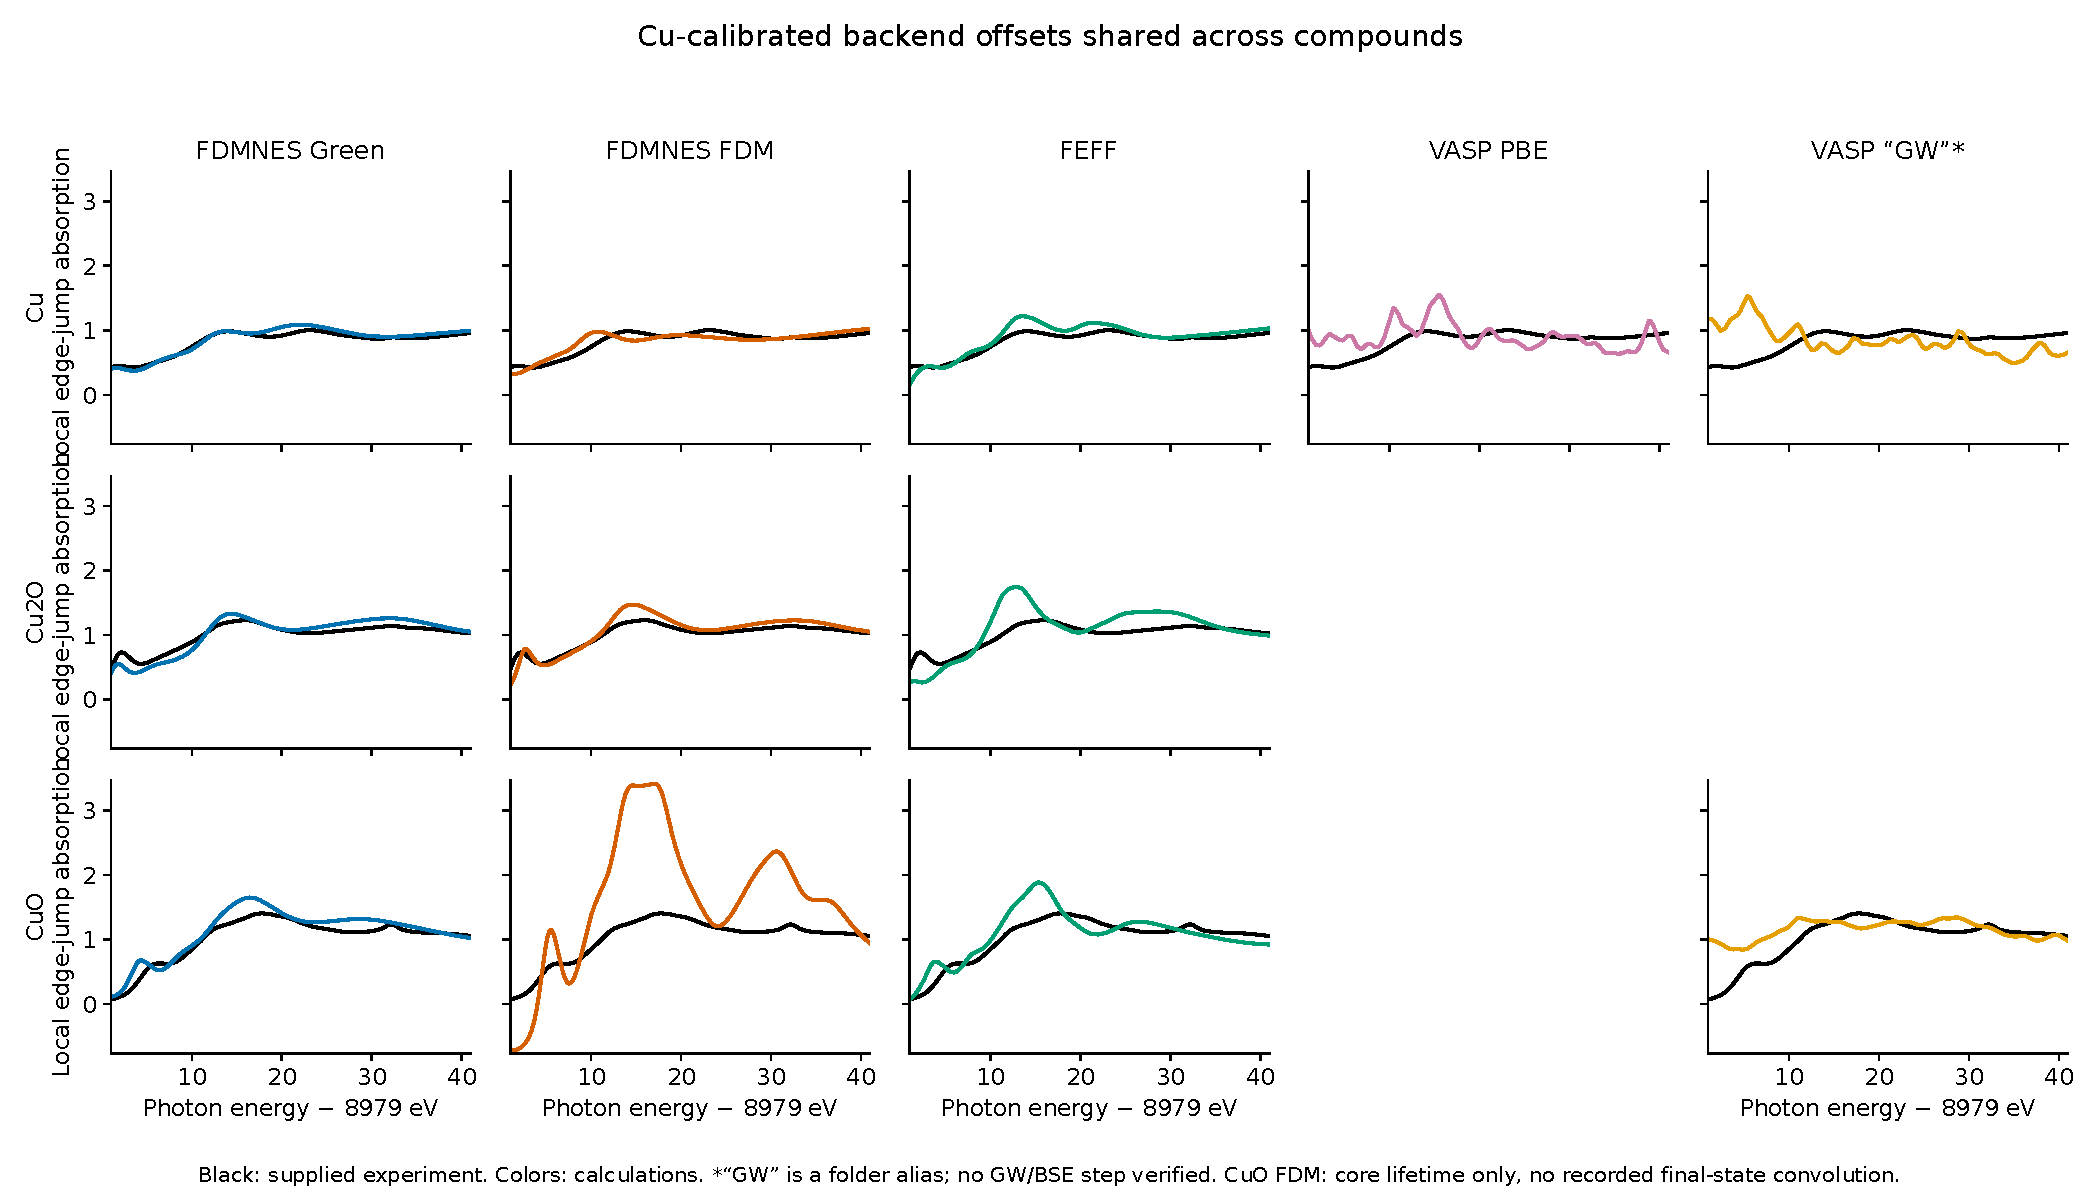
\includegraphics[width=.98\linewidth]{figures/SI_reference_grid_common.pdf}
\caption{Complete three-material, five-computation grid on common Cu-calibrated backend axes. Experiment is black and each method has a consistent color. Blank slots are missing numeric calculations. ``GW'' is an input-directory alias. CuO FDM has no recorded native final-state convolution. All plotted arrays and native inputs are supplied.}
\end{figure}
\end{landscape}
\clearpage
\begin{landscape}
\begin{figure}[p]
\centering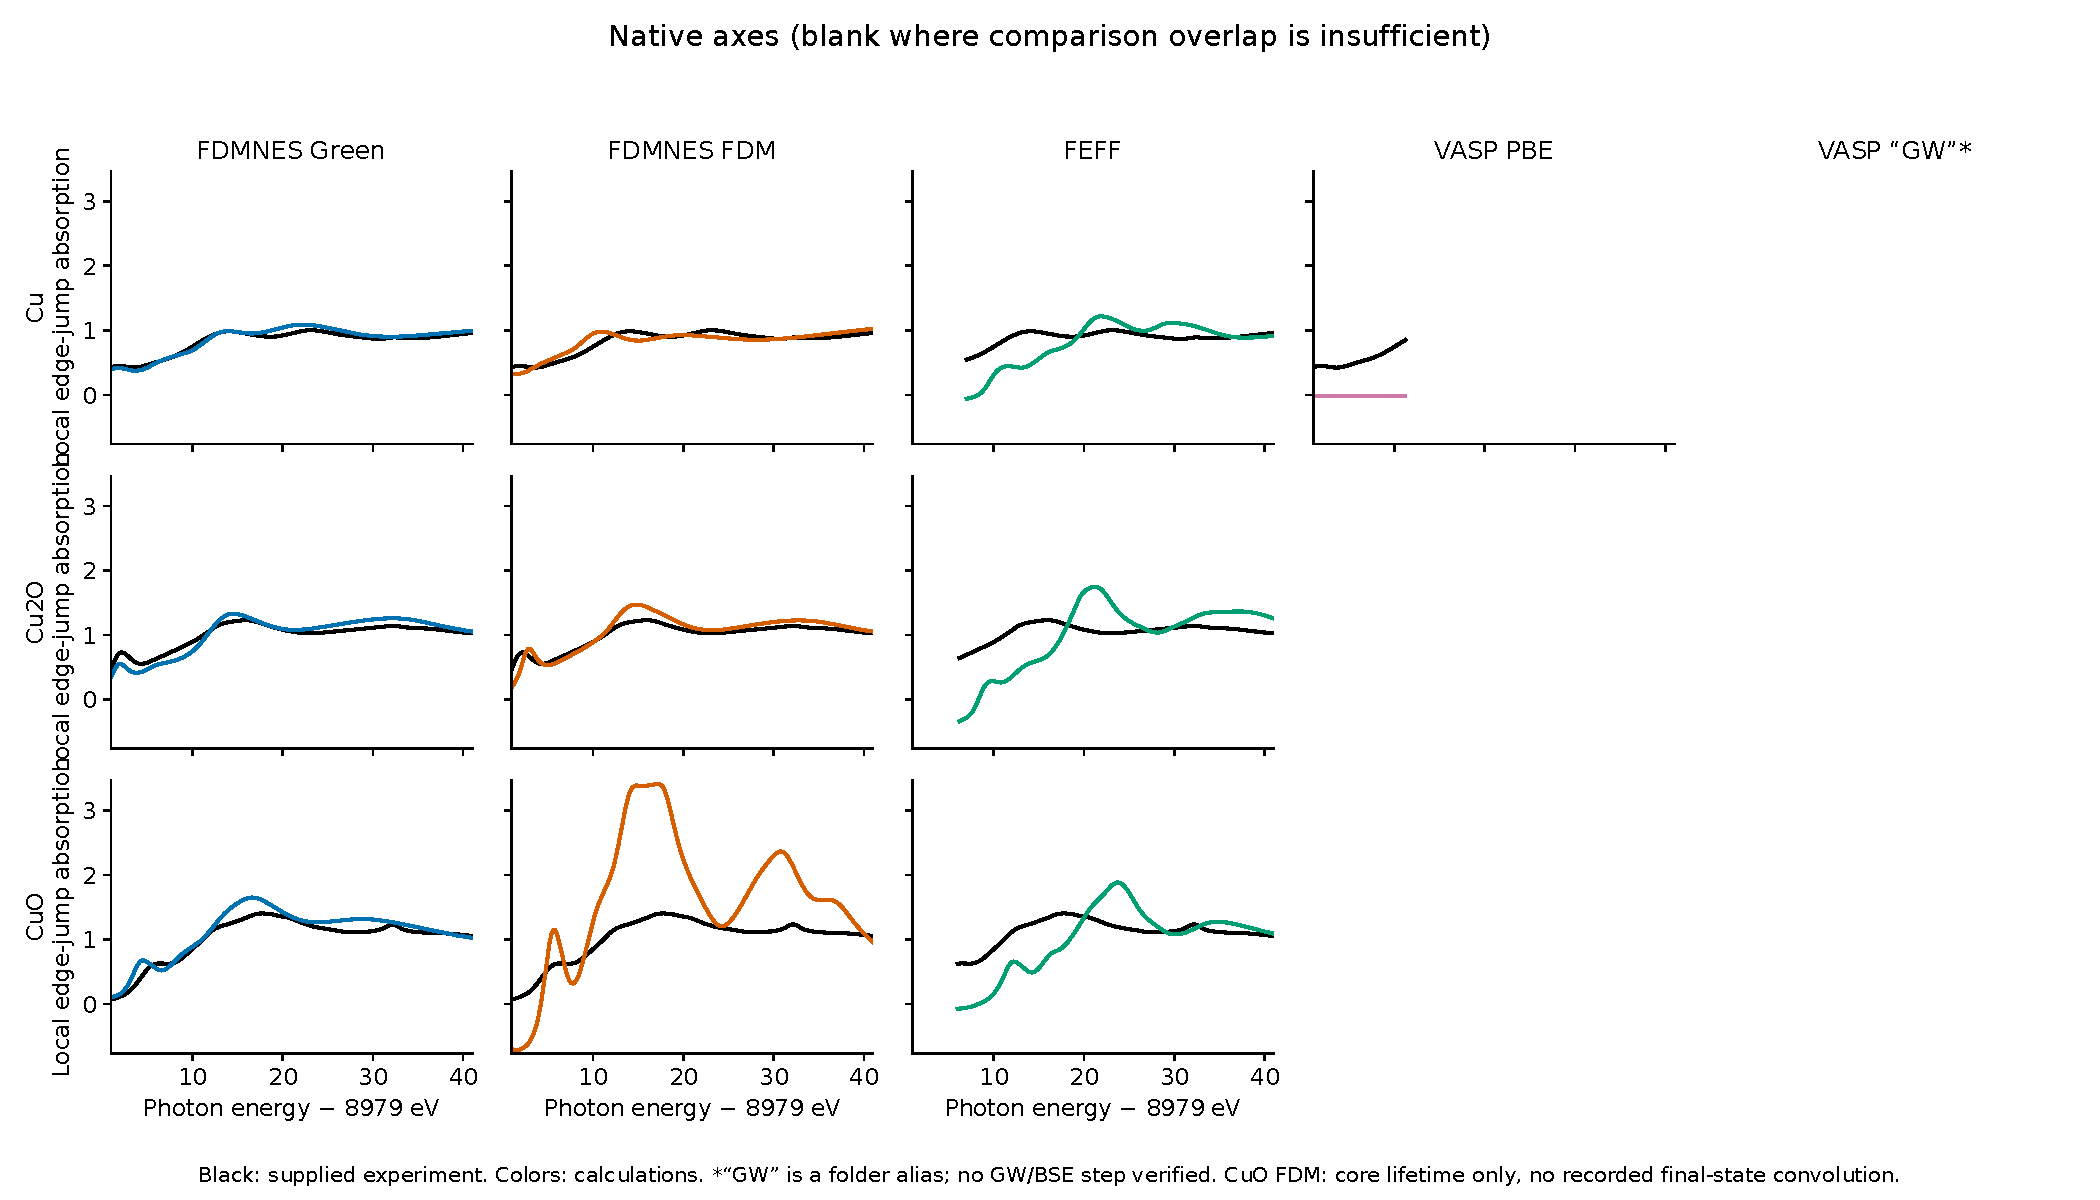
\includegraphics[width=.98\linewidth]{figures/SI_reference_grid_native.pdf}
\caption{Native input axes with zero fitted shift. Only supported intersections are compared. Blank cells also include insufficient overlap. VASP core-excitation axes lack absolute photon calibration; a small tail-only overlap is not evidence of an accurate edge.}
\end{figure}
\end{landscape}
\clearpage
\begin{landscape}
\begin{figure}[p]
\centering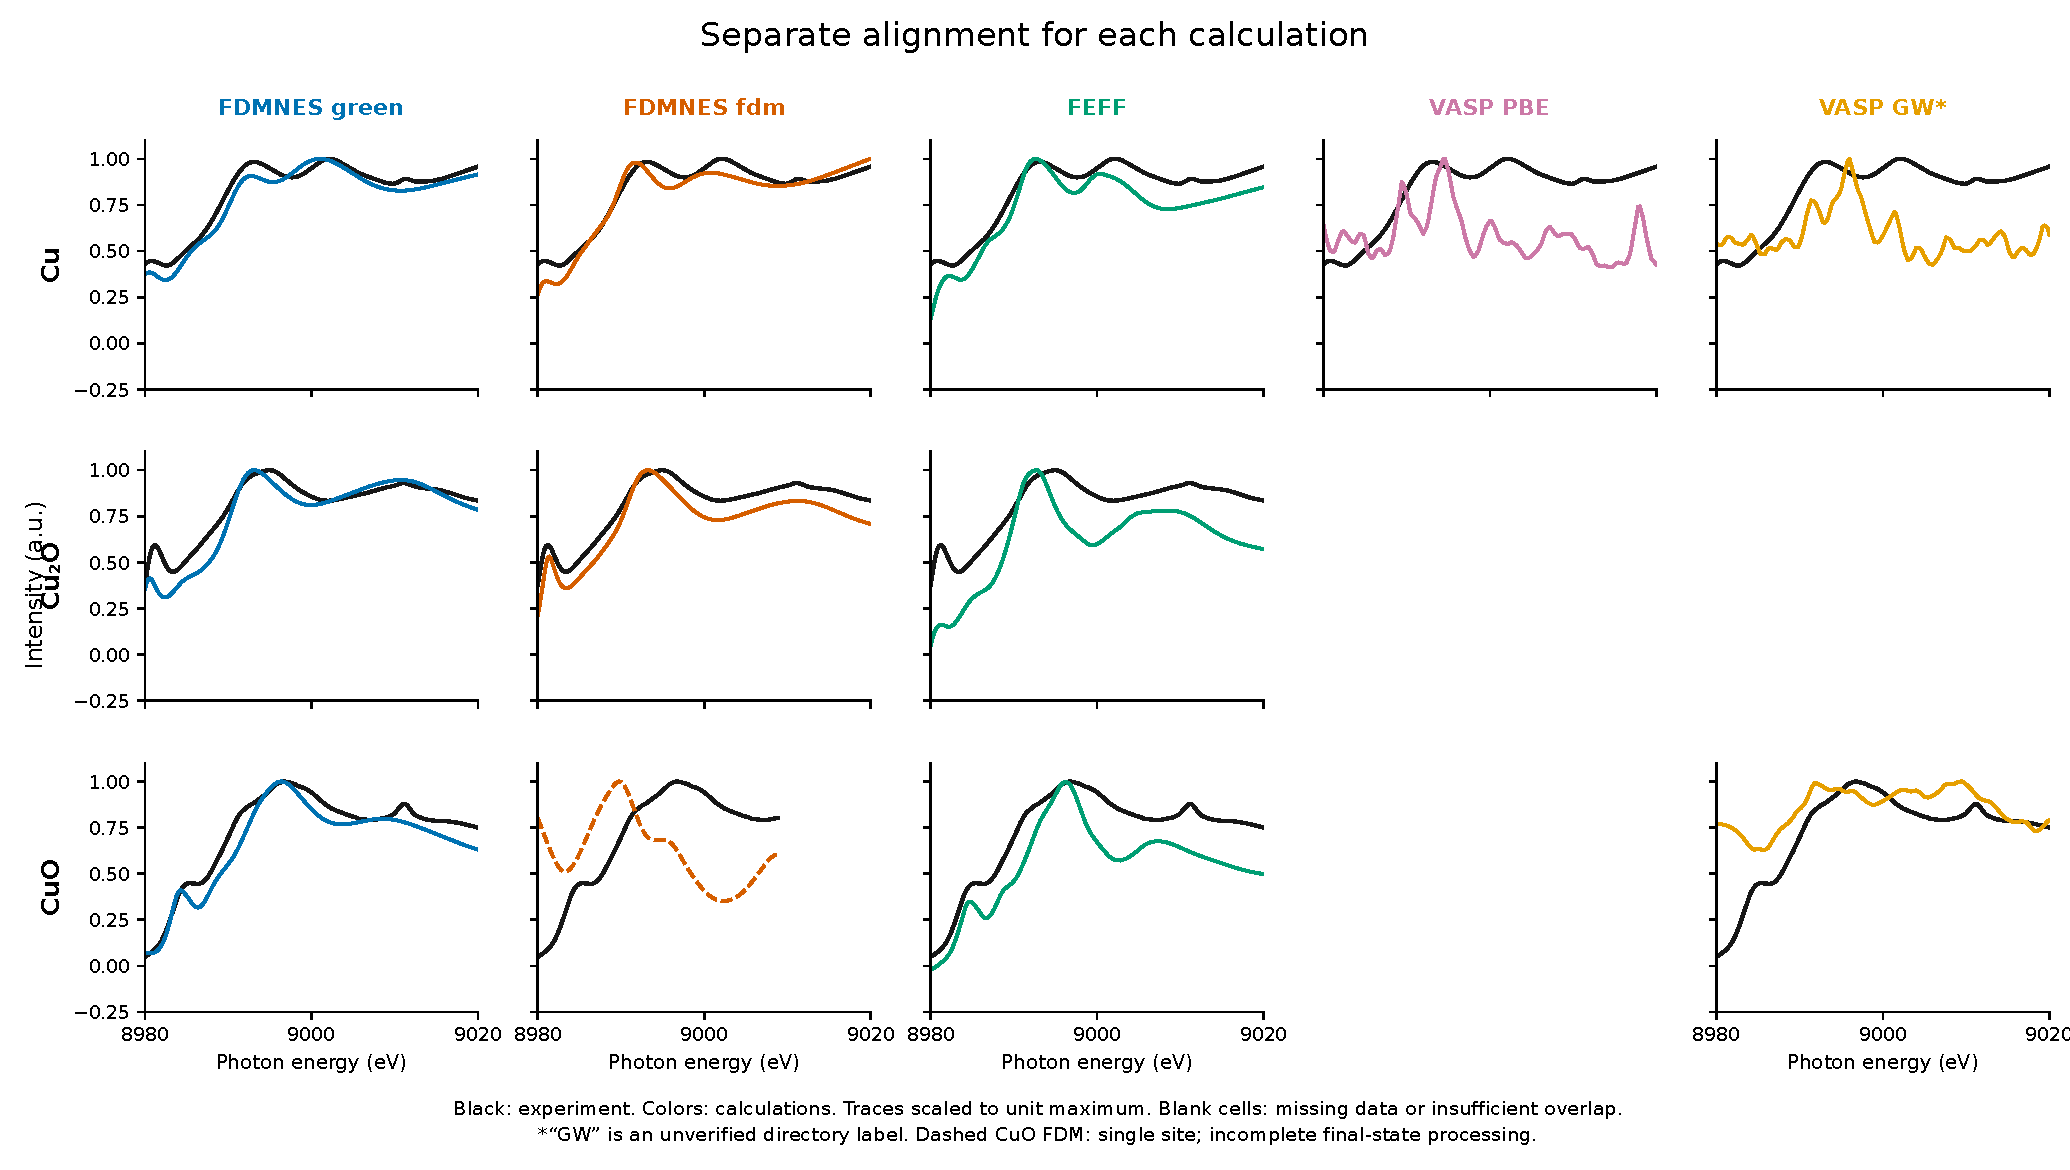
\includegraphics[width=.98\linewidth]{figures/SI_reference_grid_shape_aligned.pdf}
\caption{Separately fitted shape alignment, one bounded residual shift per available compound/method. This view removes chemical shifts and is distinct from the common-offset and native-axis views.}
\end{figure}
\end{landscape}
\clearpage
\begin{landscape}
\begin{figure}[p]
\centering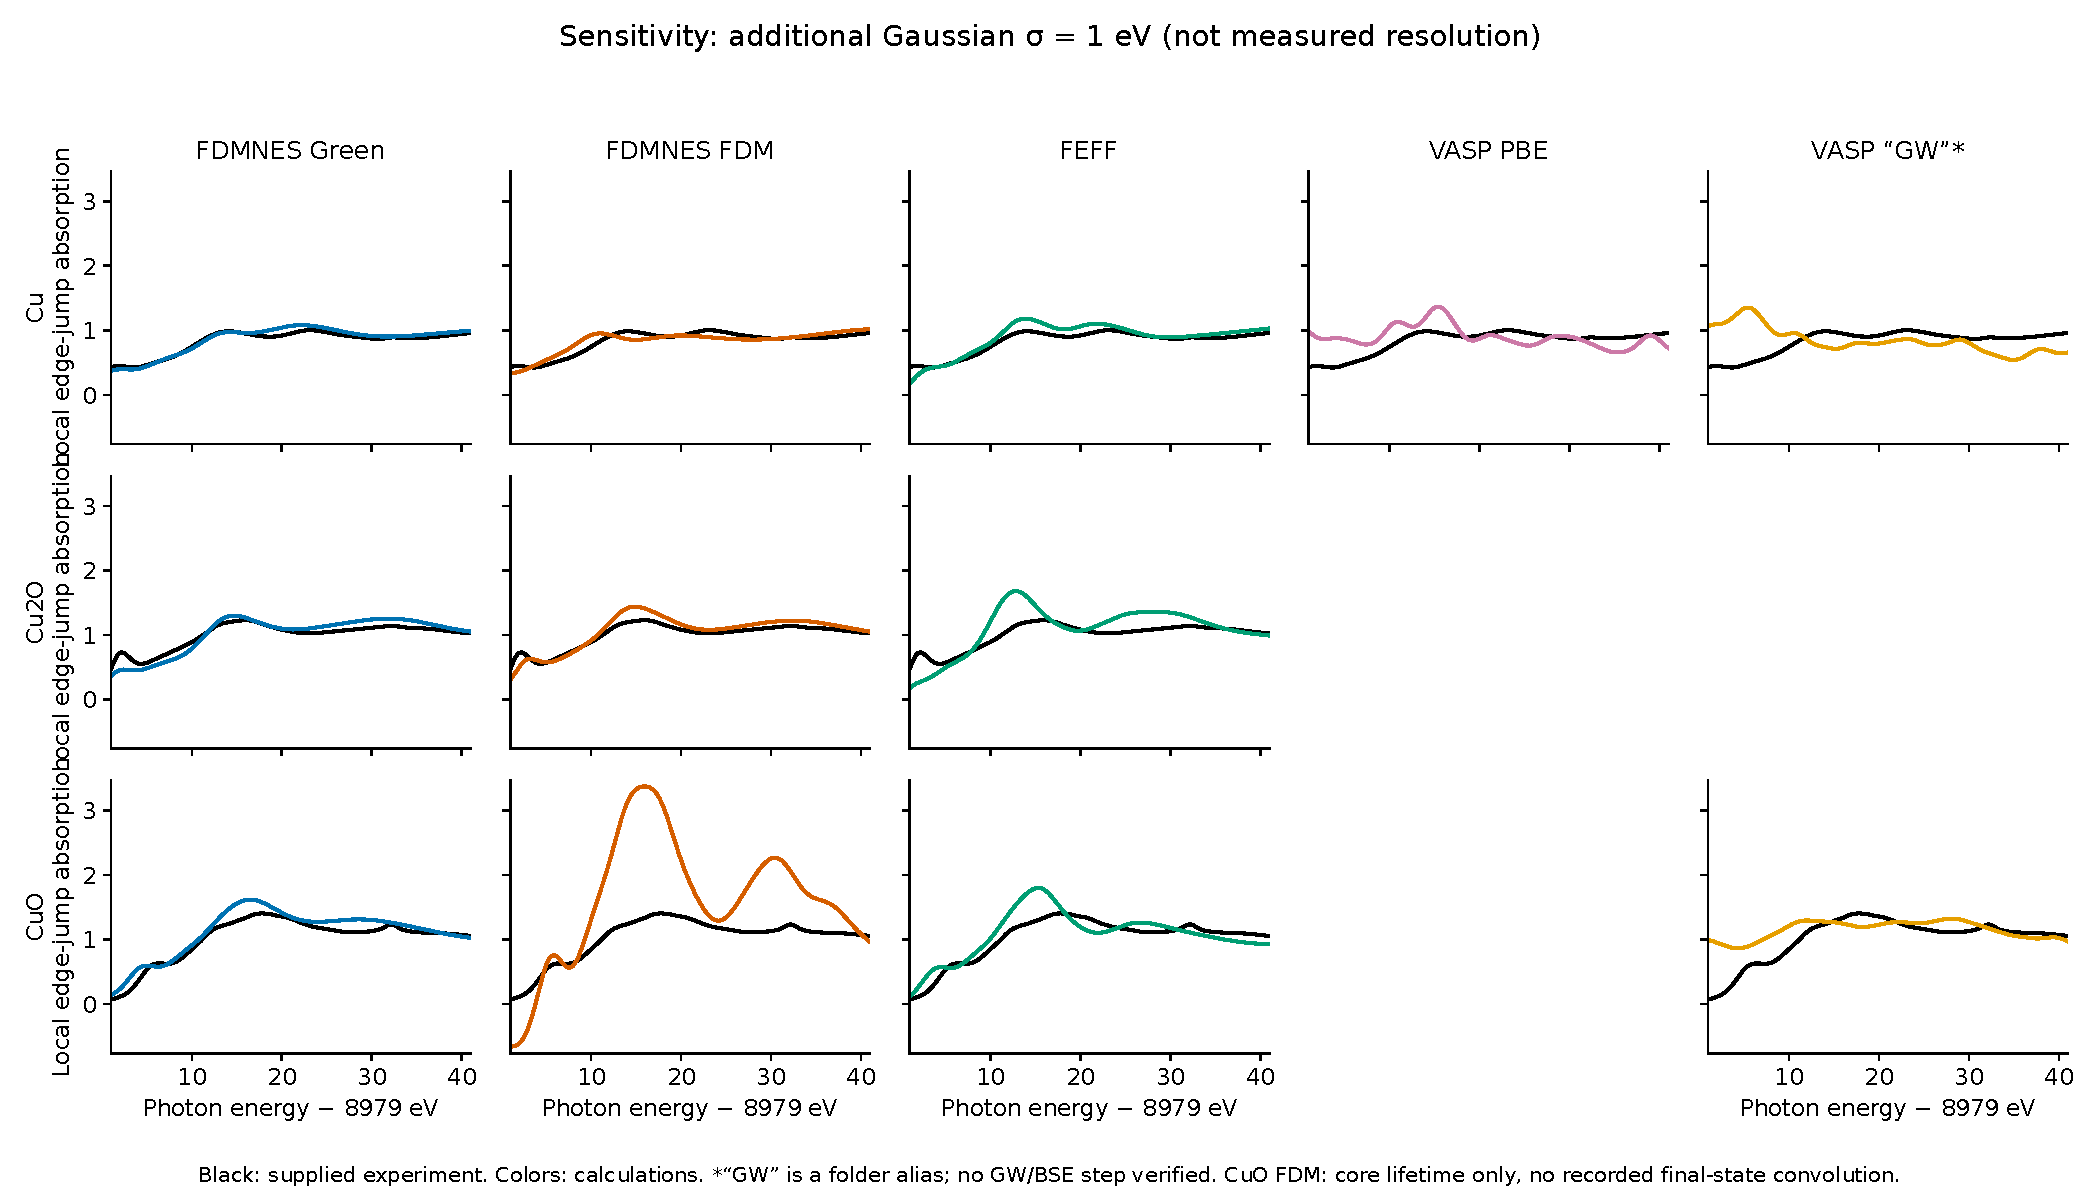
\includegraphics[width=.98\linewidth]{figures/SI_reference_grid_sigma1_sensitivity.pdf}
\caption{Sensitivity to the original notebook's additional Gaussian $\sigma=1$~eV (FWHM 2.35482~eV), at the common offsets. This width is an unvalidated sensitivity parameter, not a measured instrumental resolution. Primary native convolutions are preserved.}
\end{figure}
\end{landscape}
\clearpage
